%%=============================================================================
%% Methodologie
%%=============================================================================

\chapter{\IfLanguageName{dutch}{Methodologie}{Methodology}}%
\label{ch:methodologie}

%% TODO: Hoe ben je te werk gegaan? Verdeel je onderzoek in grote fasen, en
%% licht in elke fase toe welke stappen je gevolgd hebt. Verantwoord waarom je
%% op deze manier te werk gegaan bent. Je moet kunnen aantonen dat je de best
%% mogelijke manier toegepast hebt om een antwoord te vinden op de
%% onderzoeksvraag.





Er zullen experimenten worden uitgevoerd om de effectiviteit van verschillende mitigatietechnieken te beoordelen. Hiervoor zal een laboratoriumnetwerkopstelling worden gebruikt waarin verschillende beveiligingskwetsbaarheden worden geïntroduceerd. Het doel is om de effectiviteit van de mitigatietechnieken te evalueren bij het voorkomen of beperken van deze kwetsbaarheden. Ook worden bestaande hulpprogramma's en best practices voor het beperken van \newline IPv6-beveiligingskwetsbaarheden geëvalueerd via deze experimenten.

Om deze experimenten uit te voeren, wordt een kleinschalige laboratoriumnetwerkopstelling gebruikt met een Pfsense router, een Ubuntu LTS computer en een Windows Server met een IIS webserver. Om de experimenten uit te voeren, worden tools gebruikt uit de IPv6ToolKit, die beschikbaar zijn op \newline https://github.com/fgont/ipv6toolkit. Deze toolkit bevat verschillende tools die kunnen worden gebruikt voor het beoordelen van IPv6-beveiligingskwetsbaarheden en andere doeleinden. In dit onderzoek worden de volgende tools gebruikt:

\begin{itemize}
    \item	addr6: een IPv6 address analyse en manipulatie tool.
    \item	icmp6: een tool om aanvallen gebaseerd op ICMPv6 error berichten uit te voeren.
    \item	na6: een tool om kwaadwillige  Neighbor Advertisement berichten te verzenden.
    \item	ns6: een tool om kwaadwillige Neighbor Solicitation berichten te verzenden.
    \item	rs6: een tool om kwaadwillige Router Solicitation berichten te verzenden.
    \item	scan6: een IPv6 address scanning tool.
    \item	tcp6: een tool om kwaadwillige TCP segments uit te sturen en verschillende TCP-based attacks los te laten.
\end{itemize}

De tool wordt systematisch in het netwerk losgelaten, waarbij elk onderdeel van de tool wordt gebruikt om het netwerk te scannen en aan te vallen. Vervolgens wordt geanalyseerd hoe deze activiteiten werken en wat de impact is op het netwerk, met aandacht voor de omvang van de schade. Hierbij wordt gekeken naar de downtime van het netwerk en hoe snel het probleem kan worden opgelost.
Daarna worden alle bekende mitigatietechnieken toegepast in het netwerk en wordt de tool opnieuw gebruikt om de impact te vergelijken. Hierbij wordt gekeken naar het verschil in effectiviteit van de aanval na het toepassen van deze technieken. Zo kan worden vastgesteld of de aanval daadwerkelijk wordt vertraagd of volledig wordt voorkomen.

\section{Voorbereiding}
\subsection{laboratoriumnetwerkopstelling}
Als allereerste moet het de laboratoriumnetwerkopstelling opgesteld worden.. Het testlab zal een virtuele LAN zijn die  bestaan uit een virtuele router en virtuele machines (VM’s). De virtuele LAN zorgt ervoor dat het testlab geïsoleerd is van je fysieke LAN. Zo kunnen er veilige testen uitgevoerd worden. Het testlab zal volledig daaien in een virtualbox omgeving. VirtualBox is een gratis en open-source virtualisatiesoftware waarmee gebruikers virtuele machines kunnen maken en uitvoeren op hun computer. Je kan deze gemakkelijk installeren via \newline https://www.virtualbox.org/wiki/Downloads. 

\subsection{Pfsense router}
Om te beginnen wordt er een Pfsense router als virtuele machine geïnstalleerd in VirtualBox. Pfsense is een veelgebruikte open source firewall- en routeringssoftware die op een speciale computer of virtuele machine kan worden geïnstalleerd om te fungeren als router, firewall of ander netwerkbeveiligingsapparaat. Het is gebaseerd op het FreeBSD-besturingssysteem en wordt beheerd via een webgebaseerde grafische interface, waarmee netwerkinstellingen en -configuraties kunnen worden beheerd. Met pfSense kunnen verschillende netwerkfuncties worden gerealiseerd, zoals netwerkroutering, NAT en firewallfunctionaliteit.
De Pfsense router zal fungeren als firewall, DHCP en DNS server. Indien er een aparte internetverbinding beschikbaar is, kan er een aparte fysieke netwerkkaart worden toegewezen aan de computer om het virtuele LAN te voorzien van een publiek IP-adres. Het wordt echter verondersteld dat de meeste computers hier niet over beschikken en daarom zal deze stap worden overgeslagen.
De iso file die gebruikt wordt kan gedownload worden van volgende website: https://www.pfsense.org/download/.  Kies voor volgende attributen op de website. File Type: Install, Architecture: AMD64 (or whatever), Platform: CD Image (ISO Installer), voor de mirror kan je een plaats kiezen dicht in jouw buurt. Hier werd geopteerd voor Frankfurt, Duitsland. 

In virtualbox kies je voor volgende settings:
\begin{itemize}
    \item Memory size: 512MB 
    \item Create a virtual hard disk now
    \item Hard disk file type : VDI
    \item Storage on physical hard disk: dynamically allocated
    \item Onder storage word de gedownloade ISO tgeogevoegd als virtual optical Disk file
    \item Onder Network zorg je voor volgende instellingen
        \begin{itemize}
            \item Adapter 1
            \begin{itemize}
                \item Enable network adapter : on
                \item Attachted to: NAT
                
            \end{itemize}
        \end{itemize}
        \begin{itemize}
            \item Adapter 2
            \begin{itemize}
                \item Enable network adapter : on
                \item Attachted to: Internal Network (hier is het ‘testlab’)
                
            \end{itemize}
        \end{itemize}
    
\end{itemize}
Zodra de virtuele machine is opgezet, kan deze worden opgestart. Tijdens de installatie worden alle standaardinstellingen behouden. Zodra de installatie is voltooid, kan het ISO-optische bestand worden verwijderd en kan de virtuele machine opnieuw worden opgestart.
\newline

Na een succesvolle installatie kan de netwerkinterface worden toegewezen. Ga hiervoor naar optie 2 (Set interfaces IP address) in het PFsense menu. Met behulp van Autodetect worden de WAN- en LAN-interfaces automatisch toegewezen. Voor de LAN-interface wordt een statisch IP-adres toegewezen, bijvoorbeeld: 2001:db8:acad:10::1/64. Vervolgens wordt gevraagd om een DHCP-client in te stellen met een IPv6-adresreeks van 2001:db8:acad:10::1/64 tot 2001:db8:acad:10::9/64.
\newline

\subsection{LAN client}
Als tweede wordt er in het netwerk een LAN client geïnstalleerd. Deze zal een Ubuntu 14.04 LTS zijn. Ubuntu 14.04 LTS is een versie van het \newline Ubuntu-besturingssysteem met een focus op stabiliteit en ondersteuning op de lange termijn. Het is gebaseerd op de Linux-kernel en wordt ondersteund tot april 2019. 
\newline

De Unity-desktopomgeving biedt een moderne en gebruiksvriendelijke interface, samen met populaire toepassingen zoals Firefox, LibreOffice en \newline de GIMP-afbeeldingseditor. Ubuntu 14.04 LTS is ook ontworpen om gemakkelijk te gebruiken te zijn voor zowel nieuwe als ervaren gebruikers, met veel functies en tools. De ISO kan gedownload worden \footnote{https://www.releases.ubuntu.com/14.04/} . Er wordt een nieuwe virtual machine aangemaakt.
In virtualbox kies je voor volgende settings:
\begin{itemize}
    \item Memory size: 3072MB 
    \item Create a virtual hard disk now
    \item Hard disk file type : VDI
    \item Storage on physical hard disk: dynamically allocated
    \item Onder storage word de gedownloade ISO tgeogevoegd als virtual optical Disk file
    \item Onder Network zorg je voor volgende instellingen
    \begin{itemize}
        \item Adapter 1
        \begin{itemize}
            \item Enable network adapter : on
            \item Attachted to: Internal Network (hier is het ‘testlab’)
            
        \end{itemize}
    \end{itemize}
    
    
\end{itemize}

\subsection{Windows Server}
Als derde wordt er een windows server 2019 geïnstalleerd in het netwerk. De ISO \footnote{https://www.microsoft.com/en-us/evalcenter/download-windows-server-2019} kan gedownload worden.
In virtualbox kies je voor volgende settings:
\begin{itemize}
    \item Memory size: 2048MB 
    \item Create a virtual hard disk now
    \item Hard disk file type : VDI
    \item Storage on physical hard disk: dynamically allocated
    \item Onder storage word de gedownloade ISO tgeogevoegd als virtual optical Disk file
    \item Onder Network zorg je voor volgende instellingen
    \begin{itemize}
        \item Adapter 1
        \begin{itemize}
            \item Enable network adapter : on
            \item Attachted to: Internal Network (hier is het ‘testlab’)
            
        \end{itemize}
    \end{itemize}
    
    
\end{itemize}

\section{Configuratie}
Na een succesvolle installatie hebben zowel de Ubuntu als de Windows Server een IPv6-adres gekregen binnen de DHCP-range. Het IPv6-adres van Ubuntu is \newline 2001:db8:acad:10::9 en het IPv6-adres van de Windows Server is 2001:db8:acad:10::8.

\subsection{Pfsense}
Via de Ubuntu in hetzelfde netwerk als de Pfsense router kan de webconfigurator worden bereikt via de URL https://[ 2001:db8:acad:10::1]. Wanneer de webinterface van PfSense wordt geopend, zal elke browser de gebruiker waarschuwen voor een beveiligingsprobleem vanwege het gebruik van een zelfondertekend certificaat. Dit is echter normaal en kan gewoon worden genegeerd. Als de gebruiker Firefox of een afgeleide daarvan gebruikt, kan er op "Geavanceerd" worden geklikt, vervolgens op "Uitzondering toevoegen" en "Beveiligingsuitzondering bevestigen". Er kan worden ingelogd met de gebruikersnaam "admin" en het wachtwoord "pfsense". Om de virtuele LAN verder te isoleren van het fysieke LAN, kan er een firewallregel worden toegevoegd die verkeer van LAN naar het WAN-netwerk blokkeert, met uitzondering van de internetgateway. Maak onder firwall > rules een nieuwe regel aan met volgende eigenschappen.

\begin{itemize}
    \item  Actie: Blokkeren Interface
    \item LAN Adresfamilie: IPv4+IPv6 
    \item Protocol: Elke 
    \item Bron: LAN net 
    \item Bestemming: WAN net 
    \item Beschrijving: verkeer naar extern WAN niet toestaan 
    
\end{itemize}

\begin{figure}[H]
    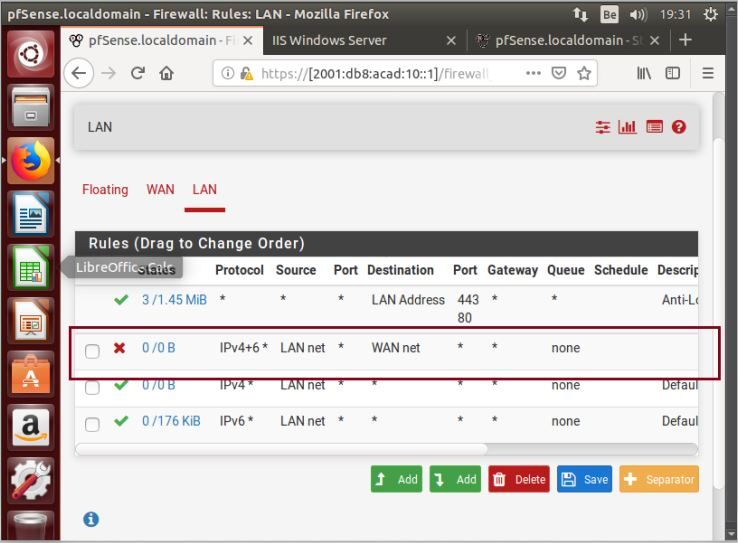
\includegraphics[scale=0.7]{Firewallrule.JPG}
    \caption{
        Een visuele weergave van de firewallregel. }
\end{figure}  

\subsection{Windows Server}

Op de Windows-server wordt een IIS-webserver geïnstalleerd om gemakkelijk te kunnen controleren wanneer de server niet meer beschikbaar is als gevolg van een aanval. Deze installatie kan eenvoudig worden uitgevoerd via de PowerShell-command line interface (CLI). 

\begin{lstlisting}[language=PowerShell,style=PowerShellStyle]
    Install-WindowsFeature -name Web-Server -IncludeManagementTools
\end{lstlisting}

\section{Uitvoering}
De volgende stap is het uitvoeren van de aanvallen vanuit de Ubuntu. Dit wordt gedaan met de IPv6Toolkit die te vinden valt op deze github \footnote{https://github.com/fgont/ipv6toolkit}: \newline . 
Je kunt de tools bouwen door het volgende commando uit te voeren:


\begin{lstlisting}[style=customStyleBashDark]
    make all
\end{lstlisting}
Je kunt de tools, het configuratiebestand, de database en bestaande handleidingen installeren door de volgende opdracht uit te voeren:

\begin{lstlisting}[style=customStyleBashDark]
    make install
\end{lstlisting}

Let op: de libpcap-bibliotheek moet al zijn geïnstalleerd op het systeem. Het overeenkomstige pakket heeft meestal de naam "libpcap-dev".

\subsection{Scanning }
Het scannen van het network kan gedaan worden met de Scan6 tool uit de IPv6toolkit. Er worden enkele scans uitgevoerd.
Er wordt hostscanning uitgevoerd op het lokale netwerk via de interface "eth0". Hierbij worden zowel ICMPv6-echoverzoeken gebruikt. De link-local adressen worden afgedrukt samen met de IPv6-adressen.

\begin{lstlisting}[language=PowerShell,style=PowerShellStyle]
    sudo scan6 \\-i eth0 \\-L \\-e \\-v
\end{lstlisting}
\begin{figure}[H]
    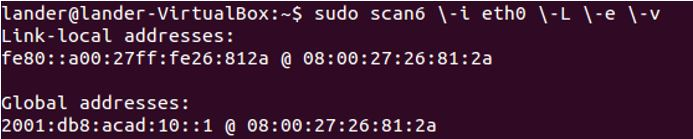
\includegraphics[scale=0.7]{Scan61.JPG}
    \caption{
       Output Scan6 op het lokaal netwerk }
       \label{fig:Scan61}
\end{figure}  

Bovendien wordt er nog een hostscanning uitgevoerd op het lokale netwerk via de "eth0" interface. Alleen globale unicast-adressen worden afgedrukt en er wordt maximaal één IPv6-adres per Ethernet-adres weergegeven. Ethernet-adressen worden samen met het bijbehorende IPv6-adres geprint.
\begin{lstlisting}[language=PowerShell,style=PowerShellStyle]
    scan6 \-i eth0 \-L \-P global \-\-print\-unique \-e
\end{lstlisting}
\begin{figure}[H]
    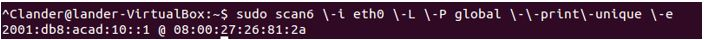
\includegraphics[scale=0.7]{Scan62.JPG}
    \caption{
        Output tweede Scan6 op het lokaal netwerk }
        \label{fig:Scan62}
\end{figure}  

\subsection{Header analyzing/manipulation }

Met de Addr6 tool kan er IPv6 adrressen  geanalyseerd worden. 


Eerst en vooral wordt de statistiek van het IPv6-adres geanalyseerd. Dit gaat met het volgende commando:

\begin{lstlisting}[language=PowerShell,style=PowerShellStyle]
    echo "2001:db8:acad:10::8" | addr6 -i -s
\end{lstlisting}
Als er meerdere IPv6-adressen geanalyseerd moeten worden, bestaat de mogelijkheid om een lijst van IPv6-adressen in te voeren in het commando. Dit ziet er dan als volgt uit:
\begin{lstlisting}[language=PowerShell,style=PowerShellStyle]
    cat MyListIPv6.txt | addr6 -i -s
\end{lstlisting}

\begin{figure}[H]
    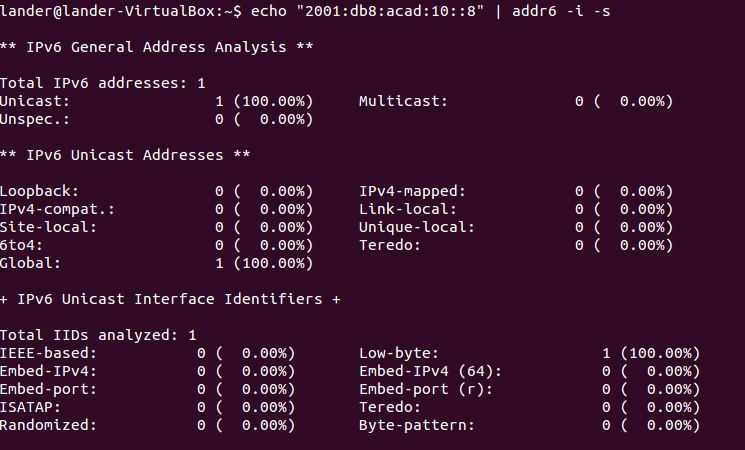
\includegraphics[scale=0.7]{StatisAddress.JPG}
    \caption{
        Output Addr6 analyze statistiek }
        \label{fig:StatisAddress}
\end{figure} 



Bij het gebruik van de Addr6 tool kunnen lijsten met IPv6-adressen gegenereerd worden. Echter, niet alle adressen in de lijst zijn mogelijk relevant of nuttig. In dergelijke gevallen kan het handig zijn om verschillende filters toe te passen om de groep IPv6-adressen te verfijnen. Deze filters kunnen onder andere het verwijderen van dubbele adressen uit de lijst, het elimineren van adressen die niet behoren tot een specifiek voorvoegsel, of het verkrijgen van adressen van een specifiek bereik omvatten. Door gebruik te maken van deze filtertechnieken wordt de resulterende lijst van IPv6-adressen meer gericht en afgestemd op de specifieke vereisten van het beoordelingsproces.

De voorbeelden worden even opgesomd: 

\begin{itemize}
    \item  Verwijder dubbele adressen:
    \begin{lstlisting}[language=PowerShell,style=PowerShellStyle]
        addr6 -i -q
    \end{lstlisting}
    \item Accepteer of blokeer specifieke prefix: 
    \begin{lstlisting}[language=PowerShell,style=PowerShellStyle]
        addr6 --accept PREFIX
    \end{lstlisting}
    \item Accepteer of blokeer adres types:
    \begin{lstlisting}[language=PowerShell,style=PowerShellStyle]
        addr6 --accept-type TYPE
    \end{lstlisting}
  \item Accepteer of blokeer adres scopes:
  \begin{lstlisting}[language=PowerShell,style=PowerShellStyle]
      addr6 --accept-scope SCOPE
        \end{lstlisting}
    \item Accepteer of blokeer unicast adres typen:
  \begin{lstlisting}[language=PowerShell,style=PowerShellStyle]
      addr6 --accept-utype TYPE
      \end{lstlisting}
\end{itemize}


\subsection{Multicast Adressen}
Met behulp van het volgende commando kan een aanval worden uitgevoerd met behulp van ICMPv6-foutpakketten:
\begin{lstlisting}[language=PowerShell,style=PowerShellStyle]
    icmp6 \-\-icmp6\-packet\-too\-big \-p ICMP6 \-d 2001:db8:acad:10::1 \-\-peer\-addr 2001:db8:acad:10::8 \-m 1240 \-v 
\end{lstlisting}

De tool genereert een ICMPv6-foutbericht van het type "Packet Too Big". Dit foutbericht adverteert een Maximum Transmission Unit (MTU) van 1240 bytes. Het wordt verzonden naar het adres "2001:db8:acad:10::1". Binnen dit ICMPv6-foutbericht wordt een ICMPv6 Echo Request-bericht opgenomen. Het bronadres van dit Echo Request-bericht is ingesteld op "2001:db8:10::1", wat hetzelfde adres is als het bestemmingsadres van het foutbericht. Het bestemmingsadres is ingesteld op \newline "2001:db8:acad:10::8". De waarden van de velden "Identifier" en "Sequence Number" van het ingebedde ICMPv6 Echo Request-bericht worden willekeurig gegenereerd. Bovendien wordt alle informatie weergegeven door het aanroepen van de verbose optie.

\begin{figure}[H]
    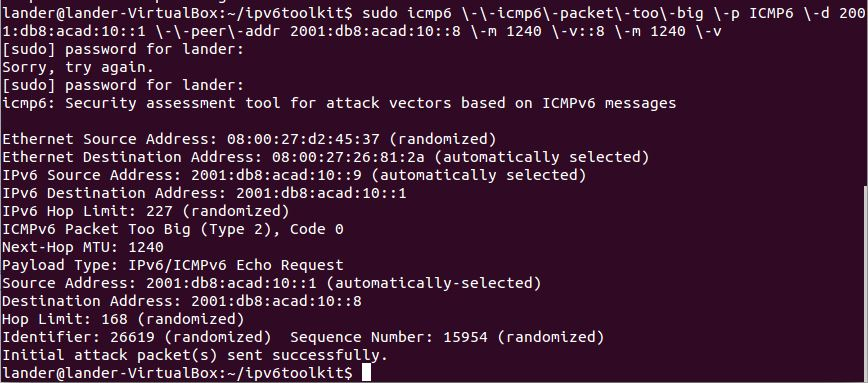
\includegraphics[scale=0.7]{ICMPcmd.JPG}
    \caption{
        Output voor de ICMPv6-aanval }
        \label{fig:ICMPcmd}
\end{figure}  

Op dit moment is het helaas nog niet mogelijk om met de huidige tool ICMPv6-content te controleren, wat betekent dat te grote pakketten nog steeds kunnen doorgaan. Deze functionaliteit is een toevoeging die nog moet worden geïmplementeerd in de IPv6-ToolKit. Gelukkig is het wel mogelijk om deze aanval te beperken door het instellen van een firewall. Door een firewall in te stellen, kunnen ongewenste pakketten worden tegengehouden en kan de netwerkbeveiliging worden versterkt.
In PFsense wordt een firewallregel ingesteld om verkeer van ICMPv6 "Packet too big" te filteren op basis van het bestemmingsadres. Vervolgens wordt de aanval opnieuw uitgevoerd. Op de figuur \ref{fig:ICMPv6} hieronder wordt de firewallregel weergegeven.

\begin{figure}[H]
    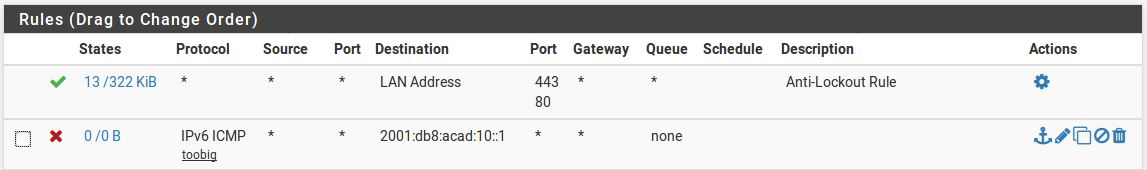
\includegraphics[scale=0.7]{FirewallTooBig.JPG}
    \caption{
        Weergave van de ICMPv6 firewallregel }
        \label{fig:ICMPv6}
\end{figure}  


\subsection{TCP}
Voordat de aanval op TCP uitgevoerd wordt, wordt er gecontroleerd of deze poort daadwerkelijk actief is met behulp van Nmap. Het volgende commando bereikt dit: 
\begin{lstlisting}[language=PowerShell,style=PowerShellStyle]
     nmap -6 -p 80 2001:db8:acad:10::8 
\end{lstlisting}
 Op de onderstaande foto zie je de uitvoer en het bewijs dat de poort inderdaad actief is.
 \begin{figure}[H]
     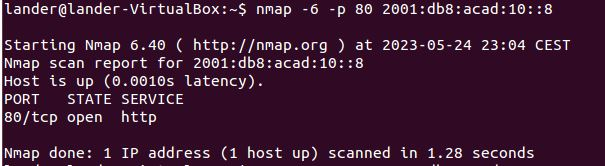
\includegraphics[scale=0.6]{NmapUP.JPG}
     \caption{
         Output voor de Nmap port 80 }
         \label{fig:Nmap1}
 \end{figure}  
 
 Vervolgens wordt de TCP-SYN-aanval uitgevoerd met het volgende commando:
\begin{lstlisting}[language=PowerShell,style=PowerShellStyle]
     sudo tcp6 -s 2001:db8:acad:10::/64 -d 2001:db8:acad:10::8 -a 80 -X S -F 100000 -l -z 1 -v
\end{lstlisting}
 \begin{figure}[H]
    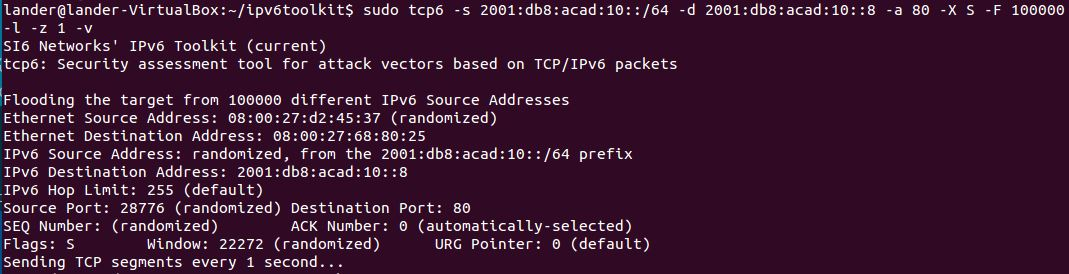
\includegraphics[scale=0.7]{TCPattack.JPG}
    \caption{
        Output van de TCP-aanval }
        \label{fig:TCPattack}
\end{figure}  

Deze tool lanceert een SYN-flood aanval op poortnummer 22 van de host \newline 2001:db8:acad:10::8. Het maakt gebruik van het netwerkinterface "eth0" en stuurt SYN-segmenten vanaf het prefix 2001:db8:acad:10::/64 naar poort 80 op het doeladres 2001:db8:acad:10::8. De tool verzendt TCP-segmenten vanaf 100.000 verschillende adressen met een interval van één seconde. Bovendien wordt de verbose optie gebruikt, zodat de tool gedetailleerde informatie zal tonen.

Tijdens de aanval kan opnieuw een Nmap-scan worden uitgevoerd, waarbij wordt aangegeven dat de poort als inactief wordt beschouwd. Dit bevestigt het succes van de aanval.

 \begin{figure}[H]
    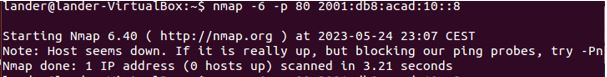
\includegraphics[scale=0.7]{NmapDOWN.JPG}
    \caption{
        Output voor de Nmap port 80 tijdens de aanval }
        \label{fig:Nmap2}
\end{figure}  

Als de aanval wordt uitgevoerd op een Ubuntu-systeem, kunnen SYN-cookies gemakkelijk worden ingesteld. Dit kan worden gedaan door het bestand sysctl.conf te openen met het volgende commando.

\begin{lstlisting}[language=PowerShell,style=PowerShellStyle]
    sudo nano /etc/sysctl.conf
\end{lstlisting}
Vervolgens worden de volgende vier regels aan het bestand toegevoegd en wordt het opgeslagen.
\begin{itemize}
     
    \item  net.ipv4.tcp\_syncookies = 1
    \item  net.ipv4.tcp\_synack\_retries = 3
    \item  net.ipv4.tcp\_max\_syn\_backlog = 2048
    \item  net.ipv4.tcp\_syncookie\_max\_age = 120
    
\end{itemize}


Het instellen van "tcp\_synack\_retries" zorgt ervoor dat er slechts drie \newline SYN/ACK-herkansingen plaatsvinden voordat een verbinding wordt opgegeven. \newline "tcp\_max\_syn\_backlog" stelt de maximale wachtrijgrootte in op 2048 verzoeken voor het ontvangen van nieuwe SYN-verzoeken. "tcp\_syncookie\_max\_age" stelt de maximale levensduur van een SYN-cookie in op 120 seconden.

Herlaad de systeemconfiguratie met de nieuwe wijzigingen:
\begin{lstlisting}[language=PowerShell,style=PowerShellStyle]
    sudo sysctl -p
\end{lstlisting}

In Windows Server is er geen specifieke configuratieoptie voor SYN-cookies, zoals beschikbaar in Linux-gebaseerde systemen. SYN-cookies zijn een mechanisme dat voornamelijk wordt gebruikt in Linux-kernels om SYN-floodingaanvallen tegen te gaan.
\newline

In Windows Server wordt de aanval echter aangepakt door firewallregels in te stellen. Dit wordt gedaan door de bronadressen van legitiem verkeer te identificeren. Dit verkeer wordt doorgelaten op poort 80, terwijl de andere IP-adressen worden geblokkeerd.

\subsection{Neighbor Discovery}

Met behulp van de ra6.1 tool kunnen diverse aanvallen worden uitgevoerd, waarbij in dit geval een flooding aanval wordt toegepast. Het commando dat wordt gebruikt om deze aanval uit te voeren, is als volgt:

\begin{lstlisting}[language=PowerShell,style=PowerShellStyle]
    sudo ra6 \-i eth0 \-s fe80::1234 \-S 08:00:27:d2:45:37 \-d FF02::1 \-N 900 \-\-flood\-dns 10#10 \-L
\end{lstlisting}

Bij deze aanval worden er 10 willekeurige IPv6-adressen van Recursive DNS-servers verzonden naar het doeladres FF02::1, waarbij elke RDNSS-optie maximaal 10 adressen bevat. Elke RDNSS-optie heeft een levensduur van 900. De pakketten worden verstuurd met een IPv6-bronadres van fe80::1234 en een Ethernet-bronadres van 00:01:02:03:04:05. Nadat het doelwit is aangevallen, wordt er geluisterd naar inkomende Router Solicitation-berichten en wordt er gereageerd met dezelfde "overstromings"pakketten.

Het bovenstaande commando demonstreert de manier waarop de ra6.1 tool wordt gebruikt om de flooding aanval uit te voeren, waarbij verschillende parameters worden ingesteld om de aanval te configureren en de gewenste effecten te bereiken.